\documentclass[9pt,twocolumn,twoside]{../../styles/osajnl}
\usepackage{fancyvrb}
\journal{i524} 

\title{D3.js}

\author[1,*]{Piyush Shinde}

\affil[1]{School of Informatics and Computing, Bloomington, IN 47408, U.S.A.}


\affil[*]{Corresponding authors: piyushsshinde1992@gmail.com}

\dates{Paper-2, \today}

\ociscodes{Document Object Model, Data Visualization, Chart}

% replace this with your url in github/gitlab
\doi{\url{https://github.com/cloudmesh/sp17-i524/blob/master/paper2/S17-IR-2035/report.pdf}}


\begin{abstract}
Data Driven Documents (D3) is a open source JavaScript library used to create dynamic, interactive visualizations on a webpage. D3 uses HTML, SVG and CSS to create visualizations with a data-driven approach to Document Object Model (DOM) manipulation, enabling users to utilize the full capabilities of modern browsers and the freedom to design the right visual interface for their data \cite{www-git}.  This paper provides a brief introduction to D3 and its various features. It also discusses D3's use cases, advantages and limitations.     
\newline
\end{abstract}

\setboolean{displaycopyright}{true}

\begin{document}

\maketitle

\section{Introduction}

Several graphical forms can be used to envision large quantitative data sets such as graphs, charts, maps and diagrams. These data sets are increasing exponentially since the advent of the World Wide Web, making the task of efficient data visualization more challenging. As a result, web browsers are considered as ideal platforms for visualizing large data sets.

Designers often employ multiple tools simultaneously for building visualisations like HTML for page content, CSS for aesthetics, JavaScript for interaction, SVG for vector graphics \cite{paper-d3}. One of the most important advantages is the uninterrupted cooperation between most of the technologies using the web as a platform, which is enabled by a document object model (DOM). The DOM reveals the ordered structure of a web page, aiding it's manipulations.  

Data Driven Documents (D3) is an open source JavaScript library, which helps in efficient manipulation of the document object models based on data. It was released in 2011 by Heer, Ogievetsky and Bostock, then part of Computer Science Department of Stanford University, Stanford, CA 94305. D3 provides a toolkit for visualizing data using web standards such as HTML, SVG, and CSS.\cite{www-git}. 

D3 resembles to document transformers such as jQuery that simplify the act of document transformation in web browsers. D3 uses the DOM’s standard SVG syntax, that shows similarities with the graphical abstractions used in graphics libraries such as Processing and Raphaël. D3 is a generalization of Protovis, and through helper modules more complex visualizations can be  achieved efficiently. 

D3's main features include selections, transitions and update, enter and exit functions. We will glance through these features in the next section.

\section{Features}
D3’s basic operand is the selection. Operators act on selections, modifying content. Data joins bind input data to elements, producing enter and exit sub-selections for the creation and destruction of elements with respect to data. Animated transitions interpolate attributes and styles smoothly over time \cite{paper-d3}.
 
\subsection{Selections}
Selections allow the user to select and manipulate HTML elements in a very simple way. D3 adopts the W3C Selectors API that contain predicates to select elements by tag, class, unique identifier, attribute, containment, or adjacency \cite{www-d3}. Unique selection methods like union and intersection can be used on these predicates. Multiple operations can be performed after selecting an element by chaining the operations. 

D3 provides select and selectAll methods for single and multiple element selections. The former selects only the first element that matches the predicates, while the latter selects all matching elements in document traversal order \cite{paper-d3}.

   
    
\subsection{Data}
Styles, attributes, and other properties are represented as functions of data in D3. They are simple, but powerful. D3 provides many built-in reusable functions and function factories, such as graphical primitives for area, line, and pie charts.

The data operator binds input data to selected nodes. Data is specified as an array of values such as numbers, strings or objects, and each value is passed as the first argument, along with the numeric index to selection functions. By default, data is joined to elements by index, the first element in the data array is passed to the first node in the selection, the second element to the second node, and so on. Once the data has been bound to the document, you can omit the data operator, D3 retrieves the previously-bound data. This allows you to recompute properties without rebinding \cite{www-d3}.

   
    
\subsection{Enter, Update and Exit}
D3’s Enter and Exit selections, aid users to create new nodes for incoming data and remove outgoing nodes that are no longer required.

When data is bound to a selection, each element in the data array is paired with the corresponding node in the selection. In case of fewer nodes as compared to elements of the data array, the extra data elements form the enter selection, that can be instantiated by appending to the enter selection. 

Updating nodes are the default selection—the result of the data operator \cite{www-d3}. In case of skipped enter and exit selections, D3 automatically selects only the elements for which corresponding data exists. Properties that are constant for the life of the element are set once on enter, while dynamic properties are recomputed per update \cite{paper-d3}. The initial selection can be divided into three parts: the updating nodes to modify, the entering nodes to add, and the exiting nodes to remove. Handling these three cases separately, precisely define the operations that run on each node, thereby optimizing performance and offering greater control over transitions. 


\begin{figure}[h]
\centering
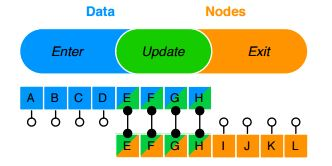
\includegraphics[scale=0.8]{images/5}
\centering
\caption{New data (blue) joining old nodes (orange) results in three sub-selections: enter, update and exit \cite{www-d3}.}
\end{figure}
   
    
\subsection{Transitions}
D3’s focus on transformation extends naturally to animated transitions. Transitions gradually interpolate styles and attributes over time. D3’s interpolators support both primitives, such as numbers and numbers embedded within strings (font sizes, path data, etc.), and compound values. D3’s interpolator registry can even be registered to support complex data structures.

D3 reduces overhead by adjusting only the attributes that change and allows greater graphical complexity at high frame rates. D3 allows sequencing of complex transitions via events. D3 does not replace the browser’s toolbox, but exposes it in a way that is easier to use \cite{www-d3}.

\section{Use Cases}

The examples tab of the official D3 website displays more than 400 examples of data visualizations, built using D3 \cite{www-gallery}. Examples include visualizations for newspapers, games, libraries and tools suggesting D3's reliability and ability to transform even the most complex data into clear visualizations. These visualizations run interactively inside web browsers and are available for anyone who wants to visualize data. 

Many of them are accompanied by a full documentation of the steps to manipulate documents based on data. The most commonly used types of data visualization are histogram, area chart, line chart, multi series line chart, bar chart, scatter-plot, pie chart, graphs, trees and maps \cite{www-gallery}. D3 also shows visualizations updating in real time.

Here are three real world examples of simplified data visualizations using D3.

\subsection{Wimbledon 2013 Data Visualisations}
This example displays a series of ten different
data visualizations of the Wimbledon tennis tournament created by Peter Cook \cite{www-cook}. The original data was collected from British tennis data
website \cite{www-tennis}.

Amongst the 10 visualizations, 3 of them include a circular match tree, a bubble chart and a horizontal histogram. The circular match tree displays concentric circles labelled as the different rounds of the Wimbledon 2013. Each concentric circle displays the player names. The result was of each match in each round is displayed by hovering the mouse over the names. The winner's name is displayed in the center of the circle.

\begin{figure}[h]
\centering
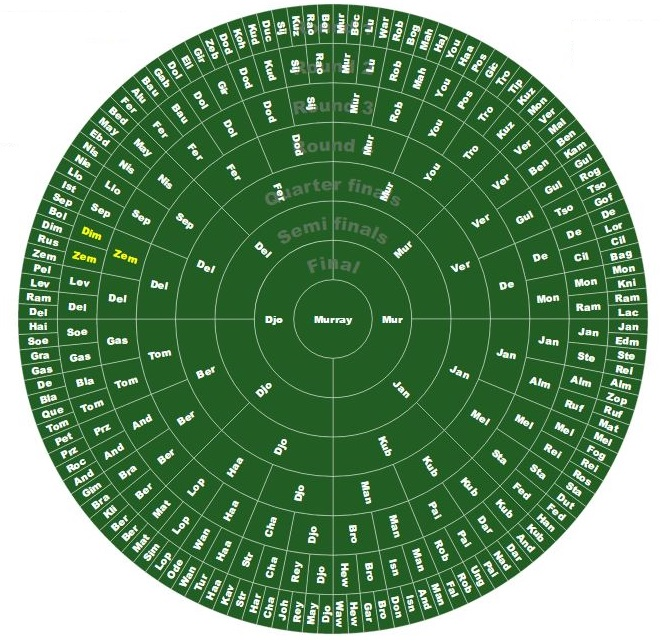
\includegraphics[scale=0.3]{images/1}
\centering
\caption{Wimbledon 2013: Circular Match Tree \cite{www-cmt}.}
\end{figure}

The bubble chart displays pair of bubbles connected by an arrow. Each arrow indicates a match where the winner had a lower ATP ranking than the loser. The size of each bubble is proportional to the ATP points of the player. Hovering the mouse over a bubble displays both the players and their ATP points with the result of the match. 

\begin{figure}[h]
\centering
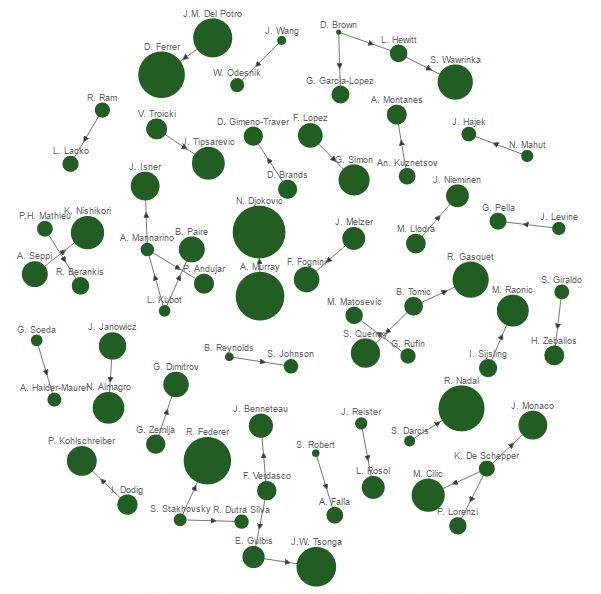
\includegraphics[scale=0.3]{images/2}
\centering
\caption{Wimbledon 2013: Bubble Chart \cite{www-bubble}.}
\end{figure}

The histogram displays the list of the top 32 players of Wimbledon 2013. It displays the number of matches won, sets won, games won and ATP ranking of all the 32 players by clicked on the respective tabs \cite{www-hist}.  

\subsection{Earthquakes in Chile since 1900}
This example helps us visualize the most important seismic events in Chile since 1900 \cite{www-map}. The earthquake data was retrieved from the ANSS Composite Catalog and joined with the Centennial Catalog from the USGS. 

 A seismic event is displayed as a circle with it's occurrence year. The radius and the color of the circles are a function of the earthquake magnitude. 

\begin{figure}[h]
\centering
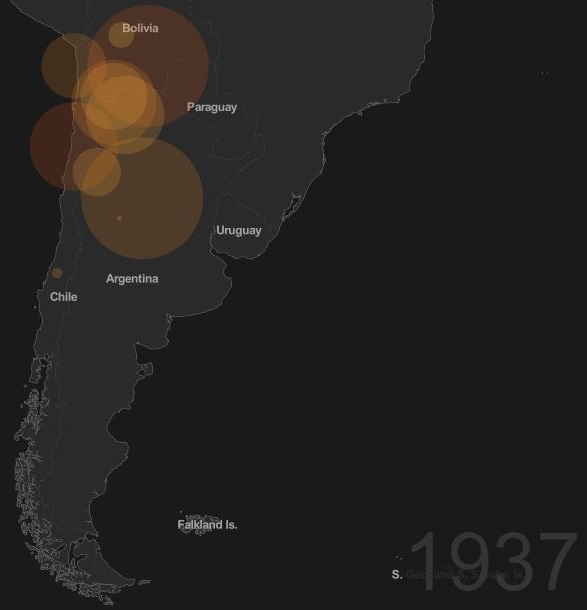
\includegraphics[scale=0.3]{images/3}
\centering
\caption{Earthquakes in Chile since 1900: Map \cite{www-map}.}
\end{figure}

\subsection{Visualizing the Racial Divide}
This example displays a visualization that highlights the impact of the segregation that exists in many US cities today based on race using d3 and force-directed maps \cite{www-fdm}. The cities include Milwaukee, Chicago, St. Louis, Syracuse, Dayton, Pittsburgh, Denver, Columbus, Kansas City, Oklahoma City, Wichita, Memphis, Baltimore and Charleston. Each city is made up of tracts from the 2010 Census.

The Census tracts are pushed away from neighboring tracts based on the change in proportion of white and black populations between each neighboring tract.

Tracts having similar racial mix as their neighbors form groups. Spaces occur where there is a significant change in the racial makeup between neighboring tracts. The space is proportional to the change in racial composition between neighbors. 

\begin{figure}[h]
\centering
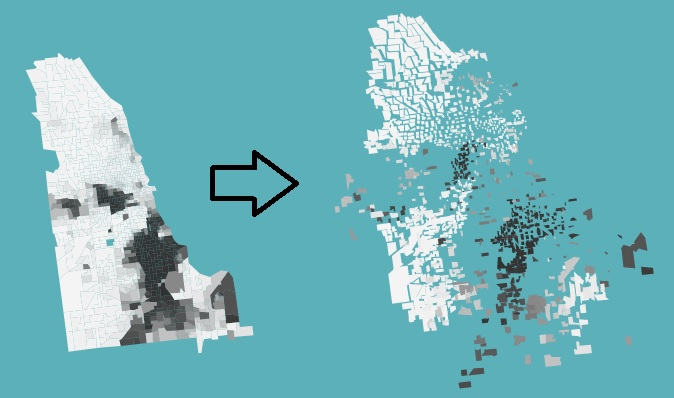
\includegraphics[scale=0.4]{images/4}
\centering
\caption{Visualizing The Racial Divide: Chicago \cite{www-chicago}.}
\end{figure}




\section{Benefits and Limitations}
D3 is an open source project, with it's source code readily available on Mike Bostock's github account \cite{www-mike}. It is free to use, which sets it apart from similar data visualization JavaScript libraries such as amCharts and FusionCharts, which need paid licenses. D3's development is supported by a big online community, where users can contribute to it's examples making it an exhaustive resource of various data visualizations. 

D3's is also a drawing library unlike conventional data visualization tool-kits, that simply create data visualizations. D3 supports dynamic visualizations, as opposed to mere static visualizations. 

D3 can be started using just one line of code, which is not the case with other data visualization tool-kits, often requiring a long installation procedure and periodic updating. D3's compatibility with web standards provide an added advantage that visualizations can be shared and viewed without the need for additional plug-ins. It is based on JavaScript which is compatible with browser’s built-in debugger. This facilitates it's fast and easy debugging.

Amongst several advantages D3 has a few limitations. It's  learning curve can be fairly steep. This is partly explained by the need for in depth knowledge of web standards, especially of SVG. Furthermore, the helper modules required for data transformations need studying too. 

Unlike JavaScript libraries such as Google Charts, D3 does not offer in-built (standard) charts. This makes it less efficient as compared to other tool-kits with custom graphs.

\section{Useful Resources}
The complete documentation of D3.js, including instructions to download and install it's latest release, examples, and several tutorials, in a systematic method are available on the main website of D3.js \cite{www-d3}. It is also a useful resource to D3's core concepts, techniques, blogs, books, courses, talks, videos and meetups \cite{www-tut}. 

The paper titled “$D^3$: Data-Driven Documents” authored by the creator of D3, compares D3 to existing web-based methods for visualization. The paper demonstrates how D3 is at least twice as fast as Protovis, through performance benchmarks. It also describes D3’s potential for dynamic visualization \cite{paper-d3}.

Another website provides a complete path to create interactive visualization using D3.js \cite{www-av}. It provides few real world examples and steps to create basic pie charts, animated bar charts and map.

\section{Conclusion}
The increasing popularity of JavaScript, has caused a major shift in the direction of web development with reduced dependencies on plug-ins. Consequently, developers are trying rely on the web browsers alone to avoid dependence on external plug-ins. This reduces the possibility of bugs or incompatibility issues as well the need to update. As an added benefit, developers can work with the existing web standards, increasing D3’s compatibility with technologies like HTML, CSS and JavaScript. This makes preparation of data visualizations easy and readily available to everyone. D3.js is an toolkit for efficiently creating complex visualizations based on large datasets. It can be used for solving real world problems by creating visualisations to better infer trends in complex large data sets.

\section{Acknowledgments}
This project was a part of the Big Data and Software and Projects (INFO-I524) course. I would like to thank Professor Gregor von Laszewski and the associate instructors for their help and support during the course. 

\bibliography{references}

\end{document}
